\section{ (30 pts)}
For a random variable $X$ whose unnormalized PDF is given as follows:
\begin{equation*}
	\tilde{f}_X(x) = x^2 \sin(2\pi x)\mathds{1}[-2 \leq x \leq 2], \quad f_X(x) = \frac{\tilde{f}_X(x)}{Z}, \quad Z:=\int_{-2}^2 \tilde{f}_x(x) \mathrm{d}x,
\end{equation*}
Using a proposal distribution with density function $q(x)$ given by
\begin{equation*}
	q(x) = \frac{3}{16}x^2 \mathds{1}[-2 \leq x \leq 2]
\end{equation*}
and $M = 16/3$,

\begin{enumerate} [(a)]
	% Problem 2(a)
	\item \label{2(a)} To sample from $q(x)$ using \verb|npr.rand| (drawing samples from $u \sim U(0,1)$), we simply employ the Inverse CDF method to sample proposal distribution with density $q(x)$ from $u$. Taking $Q(x)$ to be the CDF of the proposal distribution, we have that for $x \in [-2,2]$,
	\begin{equation*}
		\begin{aligned}
			Q(x) &= \int_{-\infty}^x q(x')\mathrm{d}x \\
			&= \frac{3}{16} \int_{-2}^x {x'}^2 \mathrm{d}x' \\
			&= \frac{1}{16} \left[{x'}^3\right]_{-2}^{x} = \frac{1}{16} \left(x^3+8\right)
		\end{aligned}
	\end{equation*}
	From the above expressions, we have thet the quantile of proposal distribution can be expressed as
	\begin{equation*}
		Q^{-1}(u) = \sqrt[3]{16u - 8}
	\end{equation*}
	Therefore, we have that
	\begin{equation*}
		u \sim U(0,1), \quad q(x):=\sqrt[3]{16u-8}
	\end{equation*}
	We also have that $E_{q(x)}[X]$, which denotes the mean of $q(x)$, expressed as
	\begin{equation*}
		\begin{aligned}
			E_{q(x)}[X] &= \int_{-\infty}^{\infty} xq(x)\mathrm{d}x \\
			&= \frac{3}{16} \int_{-2}^{2} x^3 \mathrm{d}x \\
			&= \frac{3}{64}\left[x^4\right]_{-2}^{2} = 0
		\end{aligned}
	\end{equation*}
	Similarly, we have that $\mathrm{Var}_{q(x)}[X]$, which denotes the variance of $q(x)$, expressed as
	\begin{equation*}
		\begin{aligned}
			\mathrm{Var}_{q(x)}[X] &= E_{q(x)}[X^2] - \left(E_{q(x)}[X]\right)^2 \\
			&= \int_{-\infty}^{\infty} x^2 q(x)\mathrm{d}x \\
			&= \frac{3}{16} \int_{-2}^{2} x^4 \mathrm{d}x \\
			&= \frac{3}{80} \left[x^5\right]_{-2}^{2} = \frac{12}{5}
		\end{aligned}
	\end{equation*}
	% Problem 2(b)
	\item \label{2(b)} Using the intuitions and calculations performed in \ref{2(a)}, the following code tries to draw samples from $q(x)$ and verify its correctness.
	\begin{lstlisting} [language=Python]
# draw n samples from the distribution with PDF q(x).
def rand_q(n):
	# Initialize the uniform distribution u_0 ~ U(0,1)
	u_0 = npr.rand(n)
	# Using Inverse CDF Method
	q = np.cbrt(16*u_0 - 8)
	return q

q_true_mean = 0 
q_true_var = 2.4


n = 100000
x = rand_q(n)

print(f'true mean {q_true_mean}, empirical mean {x.mean()}')
print(f'true variance {q_true_var}, empirical variance {x.var()}')
	\end{lstlisting}
	Here are the results we obtained while executing the code.
	\begin{verbatim}
true mean 0, empirical mean 0.005791076221952388
true variance 2.4, empirical variance 2.4015741588997255
	\end{verbatim}
	The negligible difference between true and empirical mean and variance here shows that the idea proposed at \ref{2(a)} works properly.
	% Problem 2(c)
	\item \label{2(c)} To sample from $f_X(x)$ with rejection sampling using $q(x)$ as a proposal with $M = 16/3$, the function \verb|rand_f_rejection| is implemented, with the correctness of the function is done by drawing histograms of samples and comparing empirical means and variances to numerically computed means and expectations done by the following code snippet.
	\begin{lstlisting}[language=Python]
# draw a sample from f_X with rejection sampling.
def rand_f_rejection():
	while 1:
		x = rand_q(1)
		u = npr.rand(1)
		crit = f_tilde(x)/(M*q(x))
		if (u < crit):
			return x

# draw samples
n = 100000
x = np.array([rand_f_rejection() for _ in range(n)])

# verification by drawing empirical distribution

plt.hist(x, bins=100, density=True, facecolor='b', edgecolor='k', alpha=0.5);

# numerical integration for the normalization constant
Z = quad(f_tilde, -2, 2)[0]
tx = np.linspace(-2, 2, 1000)
plt.plot(tx, f_tilde(tx)/Z, '-r', linewidth=2.0)

# verification by comparing mean and variances
numerical_mean = quad(lambda x: x*f_tilde(x)/Z, -2, 2)[0]
numerical_var = quad(lambda x: x**2*f_tilde(x)/Z, -2, 2)[0] - numerical_mean**2

print(f'numerical mean {numerical_mean}, empirical mean {x.mean()}')
print(f'numerical variance {numerical_var}, empirical variance {x.var()}')
	\end{lstlisting}
	Here are the results we obtained while executing the code.
	\begin{verbatim}
numerical mean 0.0, empirical mean 0.0019016832297448182
numerical variance 2.3470250033370554, empirical variance 2.3435128105756378
	\end{verbatim}
	\begin{figure}[h]
		\centering
		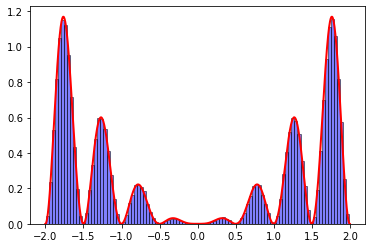
\includegraphics[width=.35\textwidth]{2(c).png}
	\end{figure}
	The negligible difference between true and empirical mean and variance here along with the histogram of samples that fits below the $f_X(x)$ shows that our algorithm works properly.
	% Problem 2(d)
	\item \label{2(d)} Now, considering the expectation $X$
	\begin{equation*}
		E\left[g(X)\right] = \int_{-2}^2 g(x)f_X(x)\mathrm{d}x = \int_{-2}^2 g(x)\frac{\hat{f}_X(x)}{Z} \mathrm{d}x
	\end{equation*}
	Using the self-normalizing importance sampling (SNIS) technique with defined $q(x)$ to estimate this expectation, the following code implements this sampling technique followed by checking the correctness for our implementation.
	\begin{lstlisting}[language=Python]
# compute the approximation for the expectation E[g(X)] using n number of samples.
# g: target function to compute expectation
# n: number of samples being used
def SNIS(g, n):
    # Draw samples from q(x)
	x = rand_q(n)
	# Calculate \omega and perform estimation
	omega = f_tilde(x)/q(x)
	mu_est = (omega*g(x)/(omega.sum())).sum()
	return mu_est


# verify your implementation using numerical integration
g = lambda x: np.log(np.abs(x) + 1.0)
n = 100000
snis_expec = SNIS(g, n)

numerical_expec = quad(lambda x: g(x)*f_tilde(x)/Z, -2, 2)[0]

print(f'Expectation via numerical integration {numerical_expec}, 
expectation via SNIS {snis_expec}')
	\end{lstlisting}
	Here are the results we obtained while executing the code.
	\begin{verbatim}
Expectation via numerical integration 0.8974560004907551, 
expectation via SNIS 0.8969511403159071
	\end{verbatim}
	The negligible difference between expectation obtained through numerical integration and SNIS shows the correctness of our algorithm with respect to the true value.
\end{enumerate}